% Based on the Template for FMI-2011 paper; to be used with:
%          fmiconf.sty - LaTeX style file, and
%          IEEEbib.bst - IEEE bibliography style file.
% --------------------------------------------------------------------------
\documentclass{article}

\usepackage{fmiconf,epsfig,graphics}
\usepackage[utf8]{inputenc}
\usepackage[hyphens]{url}
\usepackage{hyperref}
\usepackage[ngerman]{babel}

\graphicspath{{images/}} % Place images in the folder images

\title{Entwicklung eines Web Based Trainigs zum Thema Fotografie}

\twoauthors
  {A. Saskia Schreiber, B. Thomas Rehm}
	{Technische Hochschule Mittelhessen\\
	Standort Friedberg, Fachbereich IEM}
  {C. Teresa Hoffmann}
	{Justus-Liebig-Universit\"at Gie{\ss}en\\
	Fachbereich Psychologie}

\begin{document}

\maketitle

\section{Einleitung}
\label{sec:intro}

Im Rahmen der Veranstaltung \emph{Lehren und Lernen mit neuen Medien} wurde von der Psychologiestudentin Teresa Hoffmann (Justus-Liebig-Universit\"at Giessen, JLU) und den Medieninformatik-Masterstudierenden Thomas Rehm und Saskia Schreiber (Technische Hochschule Mittelhessen, THM) ein Web Based Training (WBT) zum Thema Fotografie entwickelt.

Das prim\"are Ziel des Trainings sollte die Vermittlung grundlegender Kenntnisse \"uber die Funktionalit\"at einer Kamera sein. Darauf aufbauend sollte dieTrainees Anregungen \"uber die kreative Nutzung dieser Kenntnisse erhalten.

Aus dieser Zielsetzung ergab sich folgende thematische Unterteilung:

\begin{itemize}
\item Kameratypen und ihre Unterschiede
\item Technische Grundlagen Schulung
\item Kreative Aspekte

\end{itemize}

\section{Projektorganisation}
\label{sec:orga}
Neben der inhaltlichen und technischen Umsetzung des WBT stand die interdisziplin\"are Zusammenarbeit zwischen Medieninformatik- und Psychologiestudierenden im Vordergrund. Um eine gute und m\"oglichst effektive Realisierung des WBT zu gew\"ahrleisten, wurde von Anfang an des Projektes im verteilten Team gearbeitet. Die Arbeit wurde durch den Einsatz von Tools f\"ur die kollaborative Zusammenarbeit wesentlich unterst\"utzt. Dazu sind die Google\textsuperscript{\textcopyright} Apps Documents, SpreadSheets \& Drive sowie die kollaborative Code-Versionsverwaltung GitHub verwendet worden. Die Tools wurden nicht nur f\"ur die Zusammenarbeit, sondern auch f\"ur die inhaltliche und technische Bereitstellung des WBT genutzt (siehe Abschnitt \nameref{ssec:tech}). Die Kommunikation erfolgte per Instant Messenger.

In den gemeinsamen Treffen der ersten Projektphase wurden die Projektdetails festgelegt, um einen gemeinsamen Leitplan f\"ur das Projekt zu haben. Dieser beinhaltete das inhaltliche sowie strukturelle Konzept, an dem sich das Team weitestgehend bis zur Fertigstellung orientierte.

In der zweiten Phase wurde parallel an unterschiedlichen Aufgaben gearbeitet. Texte und Grafiken wurden anhand des Leitplans erstellt, die technische und gestalterische Umsetzung des WBT wurde geplant und mit der Umsetzung in HTML, CSS und JS begonnen.
In der dritten und abschließenden Phase des Projekts wurden Inhalt und Technik zusammengef\"uhrt, Inhalte gepr\"uft und erweitert, technische Feinheiten erg\"anzt und Fehler behoben.

\section{Aspekte der Umsetzung}
\label{sec:umsetzung}
Im Folgenden wird tiefer auf die psychologischen, inhaltlichen und technischen Aspekte eingegangen, die bei der Umsetzung des WBT von Bedeutung waren. 


\subsection{Psychologische \& inhaltliche Aspekte}
\label{ssec:psy}
Bei der Konzeption des Trainings wurden verschiedene wissenschaftliche Erkenntnisse aus lern- und medienpsychologischer Forschung ber\"ucksichtigt.

Inhaltlich wurde in den Abschnitten \emph{Kameratypen} und \emph{Technische Grundlagen} zun\"achst deklaratives Grundlagenwissen vermittelt und in den anschließenden Tests abgefragt. Auf diesem Wissen baute die Lektion \emph{Kreative Aspekte} auf. Damit Lernende mit unterschiedlichem Vorwissen von dem Training profitieren k\"onnen, waren alle Hauptthemenbereiche von Anfang an zug\"anglich und nicht nacheinander freigeschaltet. Auf diese Weise werden (fortgeschrittene) Lernende nicht zu sehr in ihren Interessen eingeschr\"ankt und exploratives Lernen erm\"oglicht.

Die Tests wurden gezielt nicht nur nach Abschluss der Hauptkapitel platziert, sondern als obligatorische Zwischenpr\"ufungen nach einzelnen Themenbl\"ocken eingesetzt. Dadurch erh\"alt der Lernende direkt ein Feedback zu seinem Wissensstand und kann gegebenenfalls Inhalte erneut lesen, wenn er Teile nicht verstanden hat.

Da jedoch das Ziel war, nicht nur deklaratives Wissen, sondern die richtige und kreative Bedienung einer Kamera zu vermitteln, wurde ein Kamerasimulator integriert. Der Kamerasimulator erm\"oglicht es zum Beispiel, \"Anderungen an den Blendeneinstellungen live am Bild zu sehen. \"Uber einen Button konnte so jederzeit das Gelernte ausprobiert und dadurch in prozedurales Wissen transferiert werden. 

Bei der Erstellung der Inhalte wurde auf die gute Verst\"and\-lichkeit der Texte geachtet. Als Orientierung diente dabei das \emph{Hamburger Verst\"andlichkeitskonzept} von Langer, Schulz von Thun und Tausch (2006)\cite{rey2009e-learning}, laut dem sich verst\"andliche Texte durch vier Merkmale auszeichnen: Einfachheit, Gliederung und Ordnung, K\"urze und Pr\"agnanz und anregende Zus\"atze. Weiterhin wurde eine informelle Sprache und pers\"onliche Anrede benutzt, was nach dem Personalisierungsprinzip der kognitiven Theorie multimedialen Lernens (Cognitive Theory of Multimedia Learning von Richard E. Mayer)\cite{rey2009e-learning} das Lernen erleichtert. 

Zur besseren Verst\"andlichkeit wurden ebenfalls viele Bilder eingef\"ugt, die die Inhalte verdeutlichen. Um dem negativen Effekt der geteilten Aufmerksamkeit (Split-Attention Effect)\cite{rey2009e-learning} entgegenzuwirken, wurden die Bilder immer direkt beim dazugeh\"origen Text platziert. 


\subsection{Technische Aspekte}
\label{ssec:tech}
Die technische Grundlage des WBT bildet das von Studierenden der Technischen Hochschule Mittelhessen entwickelte WBT-Framework.

Um dieses Framework sinnvoll um eigene Komponenten erweitern zu k\"onnen, wurde sich f\"ur eine Einbindung als Git-Submodul\cite[S. 341 ff.]{chacon2014pro} entschieden, sodass das Hauptrepository allein aus den neu erstellen Inhalten besteht. Das hat den Vorteil, dass Updates und Bugfixes am Framework ohne Konflikte in das Projekt integriert werden k\"onnen. Auch mit den in diesem Kapitel erl\"auterten Erweiterungen wurde so verfahren, sofern es sich um Fremdcode handelt.

Um die Ver\"offentlichung des WBT so direkt und unkompliziert f\"ur die Entwickler zu machen, wurde sich f\"ur die Nutzung des frei verf\"ugbaren GitHub Pages\footnote{\url{https://help.github.com/articles/what-are-github-pages/}} Services entschieden, der sich optimal in den bestehenden Git-Workflow einf\"ugt. GitHub hostet mit GitHub Pages kostenlos statische Webanwendungen, die Code-Projekte auf GitHub mit einer einfachen Projektpage versorgen. Pages integriert sich insofern nahtlos in den Workflow mit Git und GitHub da zur Ver\"offentlichung einer GitHub Pages Webseite lediglich der Branch “gh-pages” angelegt werden muss. GitHub crawlt jedes Repository und erstellt dann die Webseite aus dem gh-pages-Branch. Durch pushen in diesen Branch wird die neue Version im Hintergrund gebaut. GitHub Pages ist kompatibel mit Git Submodulen pr\"uft beim Build-Prozess ob alles gelingt. Treten Fehler beim Build auf, wird der Entwickler benachrichtigt.

Da das Framework aus dem DOM\footnote{\url{https://developer.mozilla.org/en-US/docs/Glossary/DOM}} der HTML-Seite die eigentliche Webanwendung (Sections, Article, Navigation, Fragemodule etc.) beim Laden generiert, m\"ussen alle Inhalte zum Zeitpunkt des Initialisierungsprozesses des Frameworks im DOM vorhanden sein. Ein solches HTML-Dokument kann schnell einige hundert Zeilen lang werden und ist damit sehr unangenehm f\"ur Redakteure mit Inhalten zu bef\"ullen und zu pflegen. 

Das Team entschloss sich die verwendenten Tools zu verwenden, um eine elegantere L\"osung zu schaffen: Der sog. ContentLoader vereint mehrere Techniken, um die Arbeit an den Inhalten zu vereinfachen. Die Funktionsweise sieht folgenden Ablauf vor:

\begin{itemize}
\item Redakteure schreiben Inhalte und Struktur in einem ver\"offentlichten Google Spreadsheet\footnote{\url{https://docs.google.com/spreadsheets/d/1U7imA8NCahaqeIT3jlz-3J-mTuRZyrYs1rUlTZsnO_M/edit?usp=sharing}}
\item Das Spreadsheet sieht folgende Spalten vor:
SectionHeadline, ArticleHeadline, ContentType, Content
\item Sections und Articles k\"onnen definiert werden
\item Verlinkung von Bildern aus einem Google Drive Ordner erfolgt \"uber Namensnennung des Bildes + Dateiendung
\item Redakteure haben zus\"atzlich mehrere ContentTypes zur Verf\"ugung: Listen (neutral, positiv, negativ), Subheadlines, Bilder (aus Drive-Ordner oder URL)

\end{itemize}

Der ContentLoader ist ein JavaScript Script\footnote{\url{https://github.com/thomasrehm/wbt-fotografie/blob/master/res/js/script.js\#L40-L99}}, das per AJAX die Inhalte aus dem Spreadsheet im JSON Format\footnote{\url{https://spreadsheets.google.com/feeds/list/1U7imA8NCahaqeIT3jlz-3J-mTuRZyrYs1rUlTZsnO_M/od6/public/values?alt=json-in-script}} l\"adt und dann in den DOM einf\"ugt. Das Script liest die Inhaltselemente linear ein und verarbeitet diese je nach ContentType.
Um den ContentLoader realisieren zu k\"onnen wurde der Initialisierungsaufruf des Frameworks vom an den GlobalEventHandler \texttt{window.load}\footnote{\url{https://developer.mozilla.org/en-US/docs/Web/API/GlobalEventHandlers/onload}} gebunden. Dieses Event wird erst ausgel\"ost, wenn alle Elemente des DOM fertig aufgebaut sind. Bisher wurde das Framework mit dem Event \texttt{document.ready}\footnote{\url{https://developer.mozilla.org/en-US/docs/Web/API/Document/readyState}} initialisiert, was vorausgesetzt hat, das die Inhalte komplett im HTML Dokument vorhanden sind.

Wie bereits in den inhaltlichen Aspekten erw\"ahnt, war es bei der Wahl des Themas Fotografie sinnvoll, eine interaktive M\"oglichkeit zum Ausprobieren der gelernten Einstellungen zu schaffen. Daf\"ur wurde die JavaScript-Applikation bethecamera\footnote{\url{http://bethecamera.com/}} verwendet, ein interaktiver HTML5-Kamerasimulator, der \"Anderungen an Kameraeinstellungen in Echtzeit an verschiedenen Beispielbildern demonstriert.

\begin{figure}[htb]
\begin{minipage}[b]{1.0\linewidth}
  \centering
\centerline{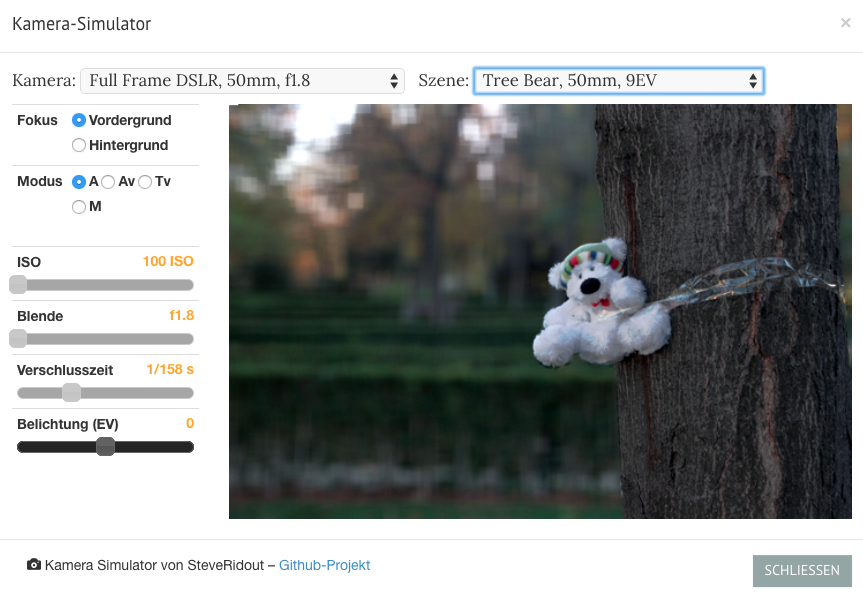
\includegraphics[width=\linewidth]{kamerasimulator.png}}
\end{minipage}
\caption{Screenshot Kamerasimulator.}
\label{fig:res}
\end{figure}

Der Simulator verwendet zum Rendern der Bilder das HTML5-Canvas-Element. Die verwendeten Bilder m\"ussen vorher entsprechend aufbereitet werden: Das Bild sollte idealerweise als HDRI (High Dynamic Range Image) vorliegen, damit \"Anderungen der Helligkeit im Simulator die gew\"unschten Effekte zeigen k\"onnen.

Zus\"atzlich muss der Vordergrund des Bildes ausgeschnitten und als PNG mit Alphakanal abgespeichert werden, damit Blureffekte der Blende sich auch wirklich nur auf den Fokuspunkt (Vorder- oder Hintergrund) auswirken.

Da die im Simulator mitgelieferten Bilder sehr gut funktionieren, wurde auf die Erg\"anzung weiterer Bilder verzichtet. Die aktuelle Umsetzung erm\"oglicht aber eine Weiterentwicklung in dieser Hinsicht.

Integriert wurde der Simulator so, dass er bei Bedarf per AJAX in ein Bootstrap-Modal\footnote{\url{http://getbootstrap.com/javascript/\#modals}} geladen wird. Das erh\"oht die initiale Ladezeit der Seite und erm\"oglicht außerdem, dass der Nutzer das aktuell aufgerufene Thema nicht verlassen muss. Gerade f\"ur das Ausprobieren zwischendurch ist dieses Kriterium essenziell.

Zuguterletzt wurde f\"ur eine optimale Pr\"asentation des Themas ein eigenes Stylesheet angelegt, welches auf dem WBT-Stylesheet aufbaut und dieses teilweise \"uberschreibt. Dadurch wird ein gewisser Wiedererkennungswert geschaffen, zumal das Standard-Theme von Bootstrap mittlerweile sehr h\"aufig im Web zum Einsatz kommt. 

\section{Reflektion}
\label{sec:reflektion}
Insgesamt ist das Projekt sehr positiv verlaufen und es gab wenige Reibungspunkte im Team zum inhaltlichem Verst\"andnis sowie der gemeinsamen Arbeit an der Umsetzung. Alle Teammitglieder sind mit dem Ergebnis zufrieden. Durch das eingesetzte WBT Framework war von Anfang an eine Struktur zur Vorgehensweise und Art der Umsetzung gegeben. Dies hat das Projekt erheblich beschleunigt, da eine Ausrichtung der Arbeitsweise und des Inhalts auf die vorgegebene Struktur notwendig war und nicht zu viel Planung f\"ur konzeptionelle Umsetzung aufgebracht werden musste.

\subsection{Aufgabenverteilung \& Wissenstransfer}
Im Rahmen des Projektes kamen wichtige bereits erworbene F\"ahigkeiten zum tragen: Die Arbeit in einem verteilten Team mit nur geringer direkter Pr\"asenz verlangt von allen Teilnehmenden koordinatorische F\"ahigkeiten und Selbstdisziplin. Das ist erwartungsgem\"aß sehr gut gelungen. Interessant war die Zusammenarbeit mit fachfremden Studierenden und somit einer ganz anderen Wissensbasis, was zu einer anderen Sichtweise auf die geplanten Features und deren Gewichtung f\"uhrte.

Leider war der Anteil neu erworbenen Wissens f\"ur beide Seiten sehr gering, da f\"ur die Entwicklung des Web Based Trainings F\"ahigkeiten aus dem Bachelorstudium Medieninformatik mehr als ausreichend waren und aufgrund der vorgegebenen Struktur des WBTs nicht alle Erkenntnisse aus Lern- und Medienpsychologie angewendet werden konnten. Der gew\"unschte Wissenstransfer stand aufgrund der inhaltlichen Ausrichtung des WBTs ebenfalls nur bedingt im Vordergrund.

\subsection{Schwierigkeiten \& Herausforderungen}
Durch die unterschiedlichen Wohnorte der Teammitglieder waren direkte Treffen nicht immer ganz einfach und mussten teilweise auch ausfallen. Daher wurde im verteilten Team oft nur virtuell mit den genannten Tools gearbeitet und parallel per Messenger kommuniziert um Probleme direkt zu kl\"aren. Durch die stressige Abschlussphase der Bachelorarbeiten der Psychologiestudierenden wurde das Projekt zeitweilig pausiert, wodurch verst\"andlicherweise der Arbeitsfluss etwas litt.

\subsection{Kritische Beurteilung des WBT Frameworks}
Der Ansatz des genutzten WBT Frameworks ist grunds\"atzlich positiv zu bewerten, da in der Theorie den Autoren eines WBT viel Arbeit abgenommen wird. Leider l\"asst die Umsetzung noch zu w\"unschen \"ubrig: Das von Bachelorstudierenden entwickelte Framework ist an vielen Stellen unfertig, unausgereift und fehleranf\"allig. 

Auch die Dokumentation ist an vielen Stellen nicht so, wie man dies erwartet. Viele Funktionen sind nicht fertig implementiert, Framework und Dokumentation geben aber den Anschein, als w\"are alles fertig. Das erschwerte die Arbeit mit dem Framework, da zun\"achst viel Einarbeitungsbedarf bestand.

Korrekturbedarf besteht auch an der grunds\"atzlichen Struktur des Frameworks: Zum Zeitpunkt der Abgabe des Projektes existierte die Basisdatei framework.js zweimal in der Dateistruktur, einmal in der Originalsource und einmal im Demo-Bereich. Kurioserweise war der Code in beiden Versionen unterschiedlich, in der Original-Source fehlte das komplette Translation-Handling der Sprachdatei.
Solche offensichtlichen Fehler sollten in einem Basistool f\"ur Projektarbeiten nicht vorkommen.

\subsection{Lessons Learned}
Die interdisziplin\"are Zusammenarbeit beeinflusste den Horizont aller Teammitglieder positiv. Alle Mitglieder haben sich mit Einsatzbereitschaft und eigenen Ideen auf das Projekt eingelassen und so zu einer guten Zusammenarbeit und einem guten Ergebnis beigetragen.



% References should be produced using the bibtex program from suitable
% BiBTeX files (here: strings, refs, manuals). The IEEEbib.bst bibliography
% style file from IEEE produces unsorted bibliography list.
% -------------------------------------------------------------------------
\bibliographystyle{IEEEbib}
\vfill
\pagebreak
%\bibliographystyle{alpha}
\bibliography{refs}

\section{Anhang}
\label{sec:anhang}
Im folgenden sind die URLs zum fertigen WBT Fotografie sowie dem Quellcode des WBT Fotografie zu finden.\\

Link zum GitHub Repository:

\noindent
\url{https://github.com/thomasrehm/wbt-fotografie}


Link zum WBT Fotografie:

\noindent
\url{http://thomasrehm.github.io/wbt-fotografie}

\noindent


\end{document}
